% Full instructions available at:
% https://github.com/elauksap/focus-beamertheme

\documentclass[aspectratio=169]{beamer}
\usetheme{focus}
\usepackage{colortbl}
\usepackage{xcolor}
\usepackage{animate}
\graphicspath{{../images/}}

\newcommand{\Lumi}{ \mathcal{L}}
\title{Normalizing Flows\texorpdfstring{\\}{,} for Particle Physics Simulations}
%\subtitle{Reducing Computational Complexity}
\institute{MIT 6.862 Team 3\\Laboratory for Nuclear Science}%\\ CLAS12 Collaboration}
\usepackage{caption}
\captionsetup[figure]{labelformat=empty}
\titlegraphic{\vspace*{0.1\paperwidth}
\includegraphics[width=0.2\paperwidth]{images/Misc/MIT-logo-black-red.png}} %{Pics/Intro/mit-clas12-combined.PNG}}
\author{Robert Johnston\texorpdfstring{\\}{,} Sangbaek Lee\texorpdfstring{\\}{,} Patrick Moran}%\texorpdfstring{\\}{,}}
%\date{\today}
\date{May 19, 2021}

\begin{document}


\begin{frame}
    \maketitle
\end{frame}

% \begin{frame}{Notes from Canvas}
% Submit your project slides on Canvas by Friday 5.14 EOD (7-15 slides: introduction, methods, results, conclusions).

% Present during your allocated session (see presentations details).

% Evaluation:
% Slides, visualization, legibility
% Delivery, clarity, timing
% Content, organization, results, questions and answers
% \end{frame}

% \begin{frame}{Outline}

%     %\vspace{-.5cm}
%          \begin{columns}[t, onlytextwidth]
%             \column{0.7\textwidth}
%                 \begin{itemize}
%                     \setlength\itemsep{2em}
%                     \item Physics background and motivation
%                     \item Normalizing Flows
%                     \item Results
%                     \item Path forward
%                 \end{itemize}
                
%             \column{0.3\textwidth}
            
%             \begin{center}
%                 \large$DV\pi^0P$ :
%                 \\~\\
%                 \large$e+p \rightarrow e'+p' + \pi^0$
%             \end{center}
                
%         \end{columns}
%     \vspace{5cm}
% \end{frame}    

\begin{frame}{Introduction: Physics Background}

    \begin{columns}
            \column{0.74\textwidth}
            \begin{itemize}
            \setlength\itemsep{1em}
                \item Particle physics experiments at Jefferson Lab\\
                \begin{itemize}
                    \item CLAS12 detector in Newport News, Virginia
                    \item highly-energetic electron beams ($e$)
                    \item stationary target protons ($p$)
                    \item Final state particles from interactions are detected
                \end{itemize}
                \item Deeply Virtual $\pi^0$ Production ( $DV\pi^0P$)
                \begin{itemize}
                    \item $e + p \rightarrow e' + p' + \gamma_1 + \gamma_2$
                    \item provides information about the 3D structure of the proton
                    \item simulation required for analysis
                    \item We will present a NF model to speed-up simulation.
                \end{itemize}
            \end{itemize}
            
             \column{0.3\textwidth}
             \centering
            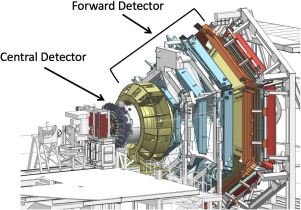
\includegraphics[width=0.26\paperwidth]{images/Detectors/overview.jpg}\\
            V.~Ziegler et al. (2020).
    \end{columns}
\end{frame}

\begin{frame}{Introduction: $DV\pi^0P$ and Simulation}
    %\vspace{-0.5cm}
    \centering
    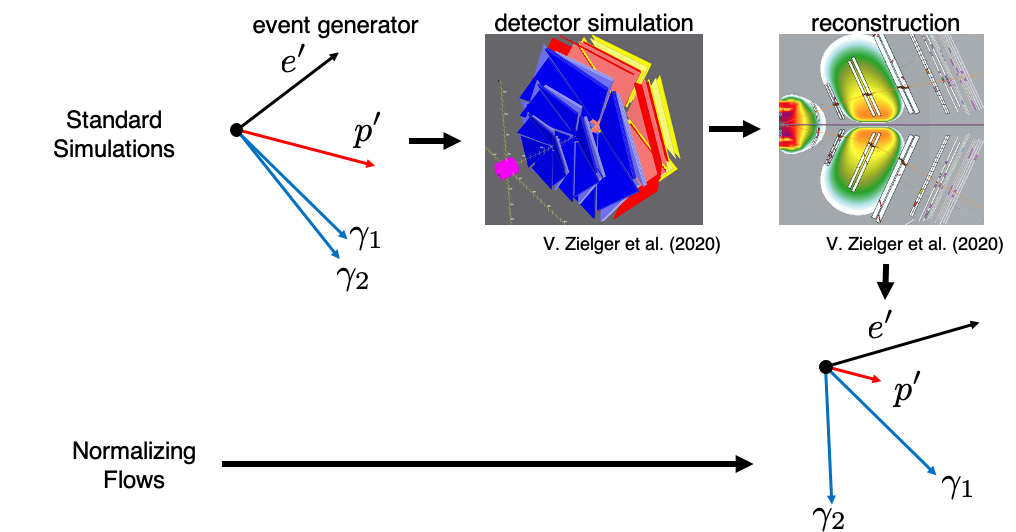
\includegraphics[width = 0.8\textwidth]{images/Detectors/simulation.png}
    %Do we need a text here? I can't think of a good one.
    % \begin{columns}
    % \column{0.65 \textwidth}
    % \begin{itemize}
    %     \item Deeply Virtual $\pi^0$ Production:\\
    %     ~~ electron + proton $\rightarrow$ electron + proton + photon + photon
    %     (DV$\pi^0$P) process provides information about the 3D structure of the proton
    
    %     \item Final state of interest includes 4 particles:\\ proton, electron, and 2 photons
    %     \item The interaction of these particles with the detector must be simulated using time-intensive Monte Carlo techniques
    %     \item Can machine learning provide speed-up for simulation?
    % \end{itemize}
    % \column{0.35 \textwidth}
    %         \centering
    %         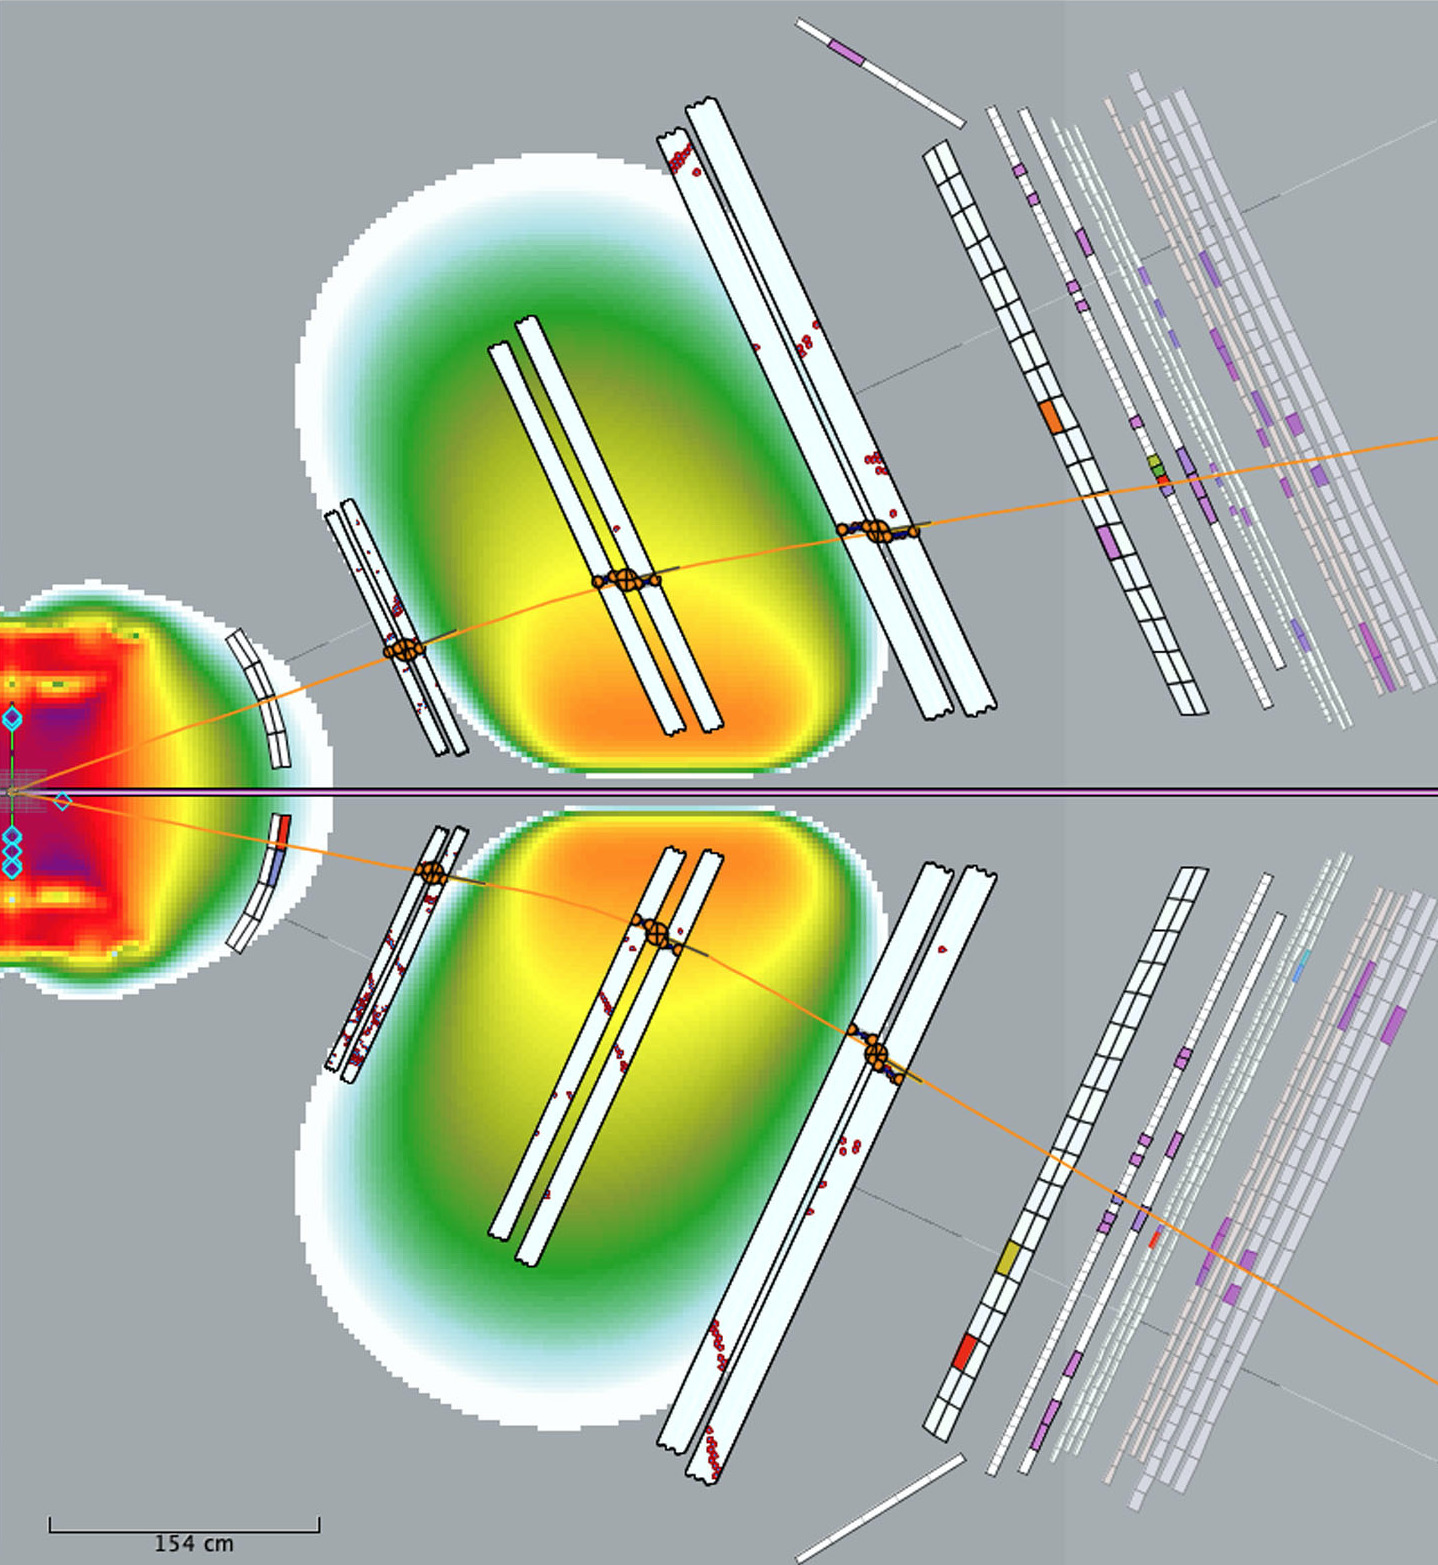
\includegraphics[width=0.35\paperwidth]{images/Detectors/ced.jpg}\\
    %         V.~Ziegler et al. (2020).
    % \end{columns}

    % $e+p \rightarrow e'+p' + \pi^0 \rightarrow e'+ p' + \gamma + \gamma$
\end{frame}

\begin{frame}{Introduction: Normalizing Flows}
    \begin{itemize}
        \item Normalizing Flow (NF) learns probability distribution $p(\mathbf{x})$ given dataset $X=\{\mathbf{x}\}$
        \item Series of transformations (flows) $g_i$ transform prior p.~d.~f. $p(\mathbf{z})$ to $p(\mathbf{x})$
        \item There are multiple NF variations, we chose UMNN-MAFs.\\
        \quad A.~Wehenkel and G.~Louppe, NeurIPS (2019)
    \end{itemize}

    \begin{columns}
        \column{0.5 \textwidth}

        \begin{align}
        \mathbf{x} =& g_N \circ g_{N-1}\circ ... \circ g_1 (\mathbf{z}) \nonumber\\
        \mathbf{z} =& f_1 \circ ... \circ f_{N-1} \circ f_N (\mathbf{x}) \nonumber \label{eqn:invertible}\\
         p(\mathbf{z_{i+1}})=&p(\mathbf{z_i})|\frac{\partial g_{i}^{-1}}{\partial \mathbf{z_i}}| \nonumber\\
         log p(\mathbf{z_{i+1}}) =& \log p(\mathbf{z_i}) + \log|\frac{\partial g_i^{-1}}{\partial \mathbf{z_i}}| \nonumber
        %  \log p(\mathbf{x}) =& \log p(\mathbf{z}) + \sum\limits_{i=1}^N \log|\frac{\partial g_i^{-1}}{\partial \mathbf{z_i}}|.
        \end{align}
        \vspace{0.1\textwidth}
        \column{0.5 \textwidth}
        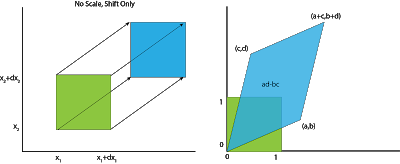
\includegraphics[width=\textwidth]{images/Misc/jacobian.png}
        blog.evjang.com/2018/01/nf1.html
    \end{columns}
    
\end{frame}



\begin{frame}{Methods: Data and architecture}
    \begin{itemize}
        \item Row: one ($e' $, $p'$, $\gamma_1$, $\gamma_2$) set. There are 5M rows.
        \item Columns: 16 features of one ($e' $, $p'$, $\gamma_1$, $\gamma_2$) set\\
        \begin{itemize}
            \item one particle has 4 features, called a "4-vector" (Energy + 3D momentum)\\
        \end{itemize}
        \item Also trained on a simplified version using only 4 of the 16 input features (electron features only).\\\vspace{0.05\textwidth}
        \item 16-feature case: 16 layers of UMNN-MAF, 32 hidden variables per layer
        \item 4-feature case: 6 layers, 80 hidden variables per layer
        \item $p(\mathbf{z})$: 16 or 4 dimensional normal distribution
    \end{itemize}
\end{frame}

% This doesn't work in overleaf
% \begin{frame}{Results: test}
% \animategraphics[autoplay,loop, height=5cm]{1}{images/400training/400training-}{0}{39}
% \end{frame}
\iffalse
\begin{frame}[noframenumbering]\centering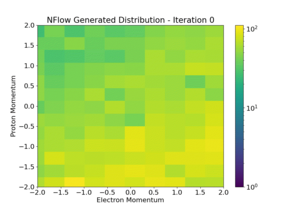
\includegraphics[width=0.8\textwidth]{images/400training/400training-0.png}\end{frame}
\begin{frame}[noframenumbering]\centering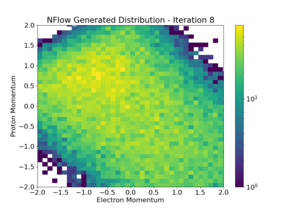
\includegraphics[width=0.8\textwidth]{images/400training/400training-1.png}\end{frame}
\begin{frame}[noframenumbering]\centering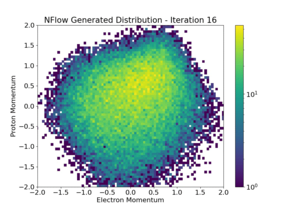
\includegraphics[width=0.8\textwidth]{images/400training/400training-2.png}\end{frame}
\begin{frame}[noframenumbering]\centering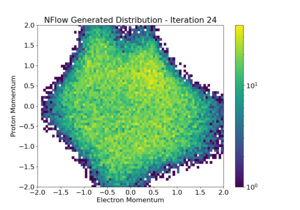
\includegraphics[width=0.8\textwidth]{images/400training/400training-3.png}\end{frame}
\begin{frame}[noframenumbering]\centering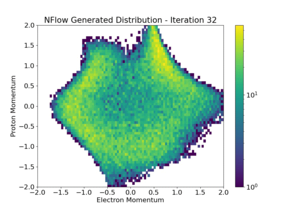
\includegraphics[width=0.8\textwidth]{images/400training/400training-4.png}\end{frame}
\begin{frame}[noframenumbering]\centering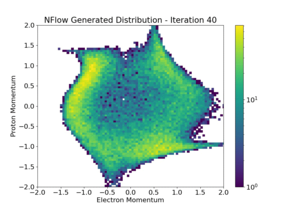
\includegraphics[width=0.8\textwidth]{images/400training/400training-5.png}\end{frame}
\begin{frame}[noframenumbering]\centering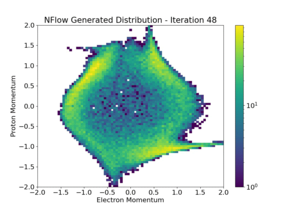
\includegraphics[width=0.8\textwidth]{images/400training/400training-6.png}\end{frame}
\begin{frame}[noframenumbering]\centering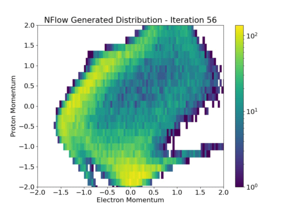
\includegraphics[width=0.8\textwidth]{images/400training/400training-7.png}\end{frame}
\begin{frame}[noframenumbering]\centering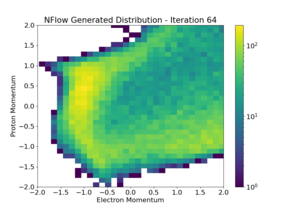
\includegraphics[width=0.8\textwidth]{images/400training/400training-8.png}\end{frame}
\begin{frame}[noframenumbering]\centering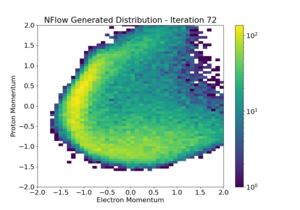
\includegraphics[width=0.8\textwidth]{images/400training/400training-9.png}\end{frame}
\begin{frame}[noframenumbering]\centering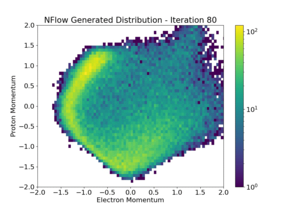
\includegraphics[width=0.8\textwidth]{images/400training/400training-10.png}\end{frame}
\begin{frame}[noframenumbering]\centering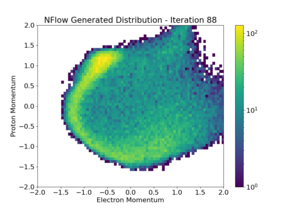
\includegraphics[width=0.8\textwidth]{images/400training/400training-11.png}\end{frame}
\begin{frame}[noframenumbering]\centering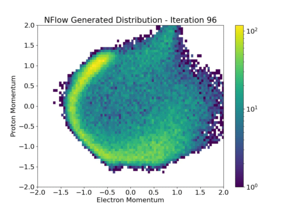
\includegraphics[width=0.8\textwidth]{images/400training/400training-12.png}\end{frame}
\begin{frame}[noframenumbering]\centering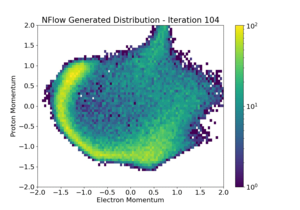
\includegraphics[width=0.8\textwidth]{images/400training/400training-13.png}\end{frame}
\begin{frame}[noframenumbering]\centering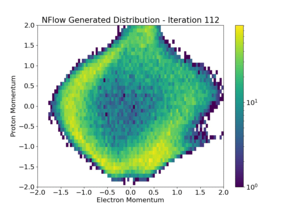
\includegraphics[width=0.8\textwidth]{images/400training/400training-14.png}\end{frame}
\begin{frame}[noframenumbering]\centering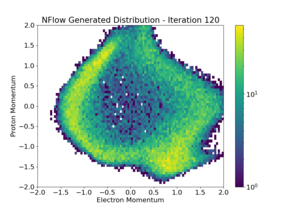
\includegraphics[width=0.8\textwidth]{images/400training/400training-15.png}\end{frame}
\begin{frame}[noframenumbering]\centering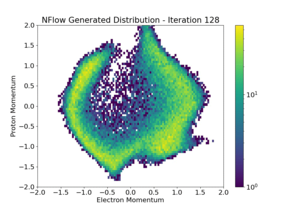
\includegraphics[width=0.8\textwidth]{images/400training/400training-16.png}\end{frame}
\begin{frame}[noframenumbering]\centering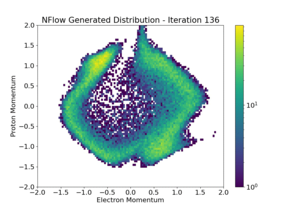
\includegraphics[width=0.8\textwidth]{images/400training/400training-17.png}\end{frame}
\begin{frame}[noframenumbering]\centering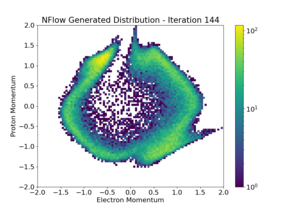
\includegraphics[width=0.8\textwidth]{images/400training/400training-18.png}\end{frame}
\begin{frame}[noframenumbering]\centering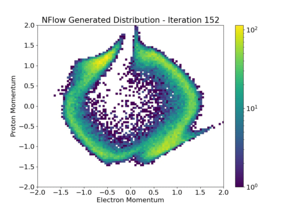
\includegraphics[width=0.8\textwidth]{images/400training/400training-19.png}\end{frame}
\begin{frame}[noframenumbering]\centering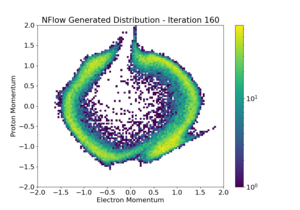
\includegraphics[width=0.8\textwidth]{images/400training/400training-20.png}\end{frame}
\begin{frame}[noframenumbering]\centering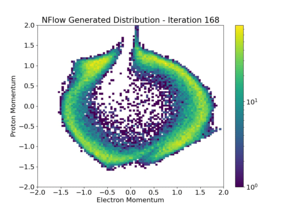
\includegraphics[width=0.8\textwidth]{images/400training/400training-21.png}\end{frame}
\begin{frame}[noframenumbering]\centering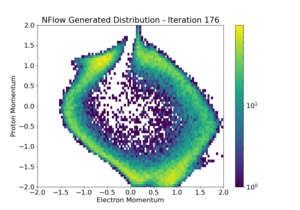
\includegraphics[width=0.8\textwidth]{images/400training/400training-22.png}\end{frame}
\begin{frame}[noframenumbering]\centering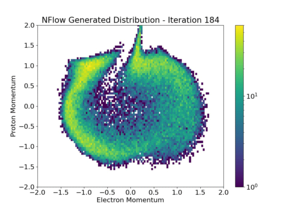
\includegraphics[width=0.8\textwidth]{images/400training/400training-23.png}\end{frame}
\begin{frame}[noframenumbering]\centering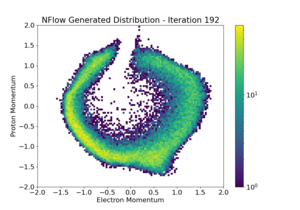
\includegraphics[width=0.8\textwidth]{images/400training/400training-24.png}\end{frame}
\begin{frame}[noframenumbering]\centering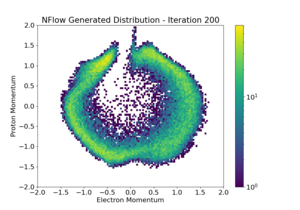
\includegraphics[width=0.8\textwidth]{images/400training/400training-25.png}\end{frame}
\begin{frame}[noframenumbering]\centering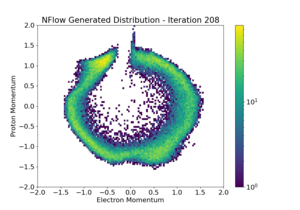
\includegraphics[width=0.8\textwidth]{images/400training/400training-26.png}\end{frame}
\begin{frame}[noframenumbering]\centering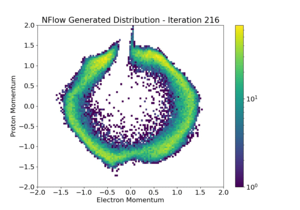
\includegraphics[width=0.8\textwidth]{images/400training/400training-27.png}\end{frame}
\begin{frame}[noframenumbering]\centering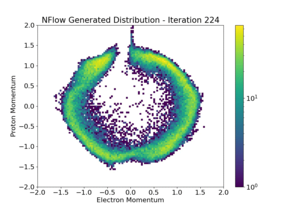
\includegraphics[width=0.8\textwidth]{images/400training/400training-28.png}\end{frame}
\begin{frame}[noframenumbering]\centering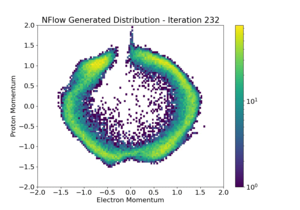
\includegraphics[width=0.8\textwidth]{images/400training/400training-29.png}\end{frame}
\begin{frame}[noframenumbering]\centering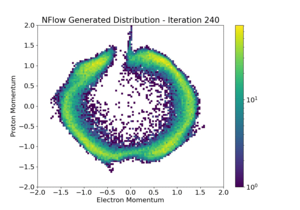
\includegraphics[width=0.8\textwidth]{images/400training/400training-30.png}\end{frame}
\begin{frame}[noframenumbering]\centering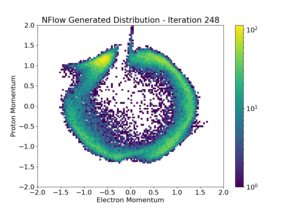
\includegraphics[width=0.8\textwidth]{images/400training/400training-31.png}\end{frame}
\begin{frame}[noframenumbering]\centering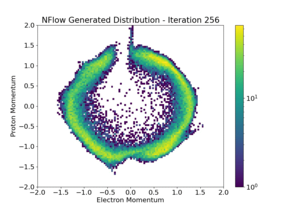
\includegraphics[width=0.8\textwidth]{images/400training/400training-32.png}\end{frame}
\begin{frame}[noframenumbering]\centering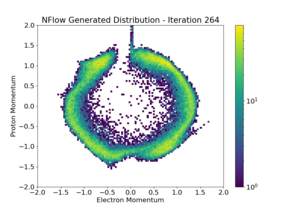
\includegraphics[width=0.8\textwidth]{images/400training/400training-33.png}\end{frame}
\begin{frame}[noframenumbering]\centering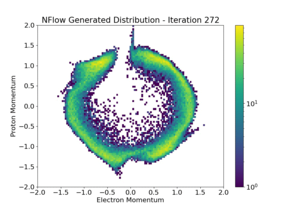
\includegraphics[width=0.8\textwidth]{images/400training/400training-34.png}\end{frame}
\begin{frame}[noframenumbering]\centering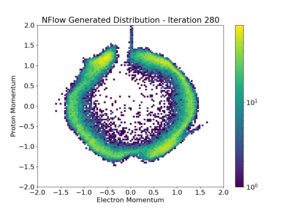
\includegraphics[width=0.8\textwidth]{images/400training/400training-35.png}\end{frame}
\begin{frame}[noframenumbering]\centering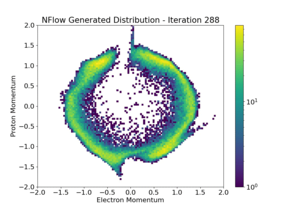
\includegraphics[width=0.8\textwidth]{images/400training/400training-36.png}\end{frame}
\begin{frame}[noframenumbering]\centering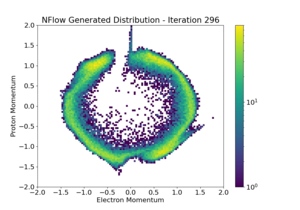
\includegraphics[width=0.8\textwidth]{images/400training/400training-37.png}\end{frame}
\fi


\begin{frame}{Results: Evaluating NF Sampled Data}
    Manually adjusted hyperparamters (previous slide) to arrive at what appeared to produce the best results:
            \begin{itemize}
                    \setlength\itemsep{0.3em}
                    \item Qualitative comparison of 1D feature distributions
                    \item Quantitative comparison of 1D feature distributions
                    \item Qualitative comparison of 2D feature distributions
                    \item Ability to recover non-trivial physics quantities
            \end{itemize}
    Sampling from the trained NF models was about $\sim$ 4 Hz for the 16-feature model and $\sim$ 200 Hz for the 4-feature model: a 10x to 500x speedup over traditional methods!
   
\end{frame}


\begin{frame}{Results: Comparing Generated and Test Distributions}
   \begin{columns}
            \column{0.3\textwidth}
            Electron Features
            \begin{itemize}
                    \setlength\itemsep{0.3em}
                    \item Energy and Z-momentum are well reproduced, except for high energy cutoff
                    \item Transverse momenta are complex and more difficult to match finely
            \end{itemize}
   
            \column{0.3\textwidth}
            \begin{figure}[H]
            \centering
            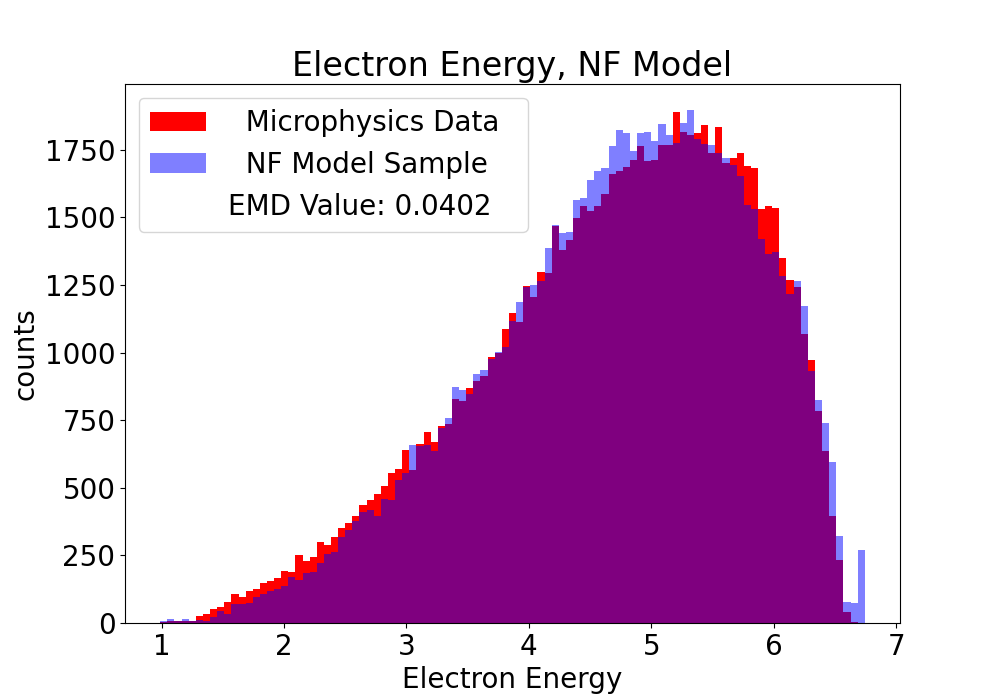
\includegraphics[width=.97\textwidth]{images/Features16/Electron_Energy,_NF_Model.png}
            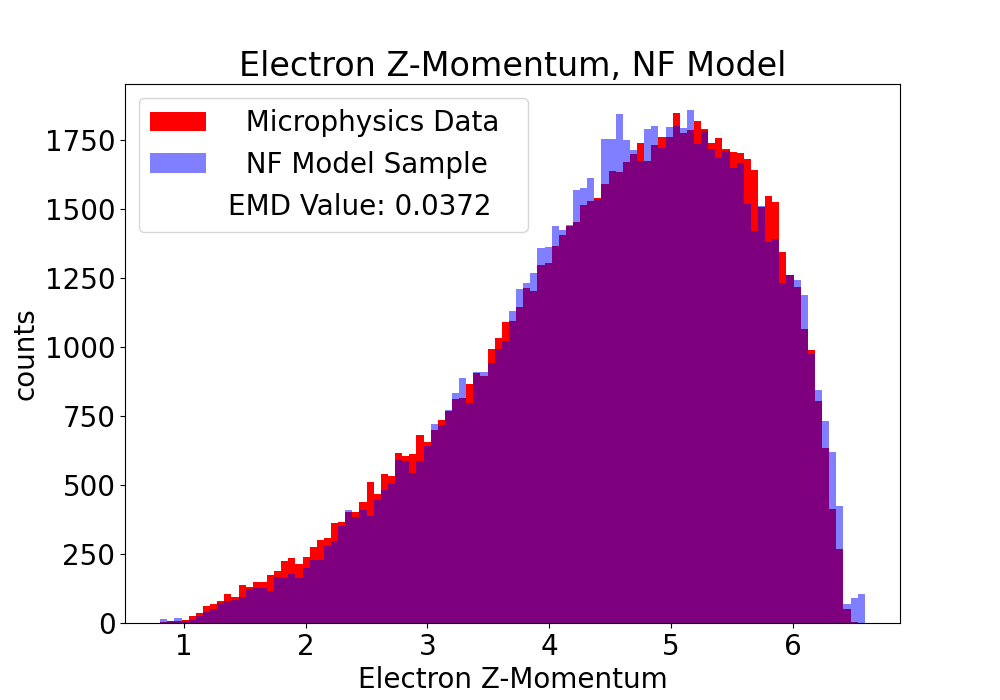
\includegraphics[width=.97\textwidth]{images/Features16/Electron_Z-Momentum,_NF_Model.png}
            \label{fig:clas6}
            \end{figure}
            
             \column{0.3\textwidth}
             \begin{figure}[H]
            \centering
            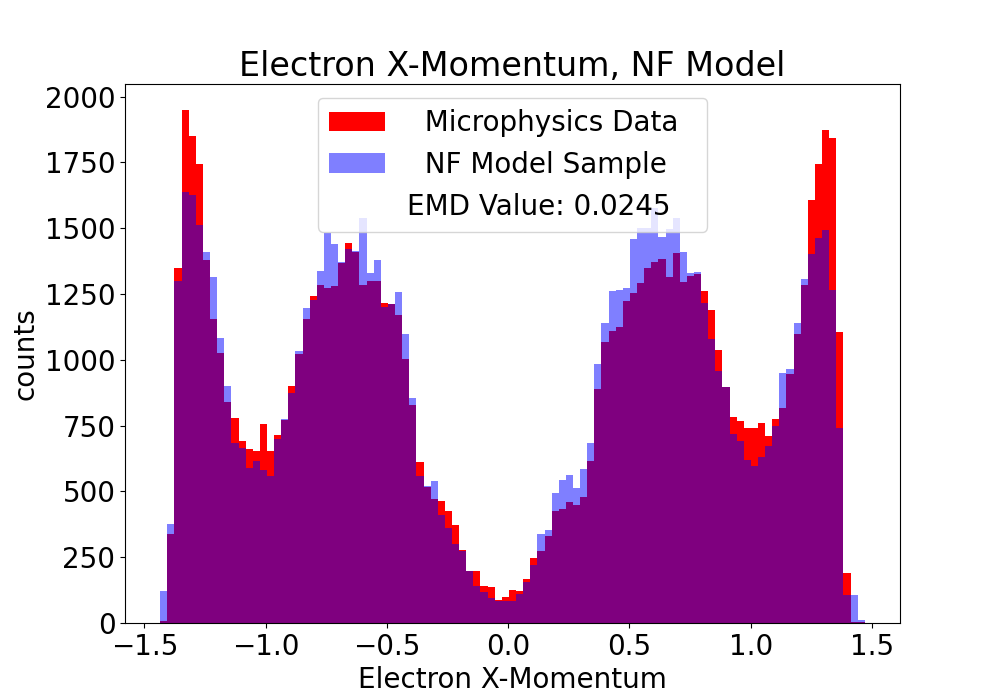
\includegraphics[width=.97\textwidth]{images/Features16/Electron_X-Momentum,_NF_Model.png}
            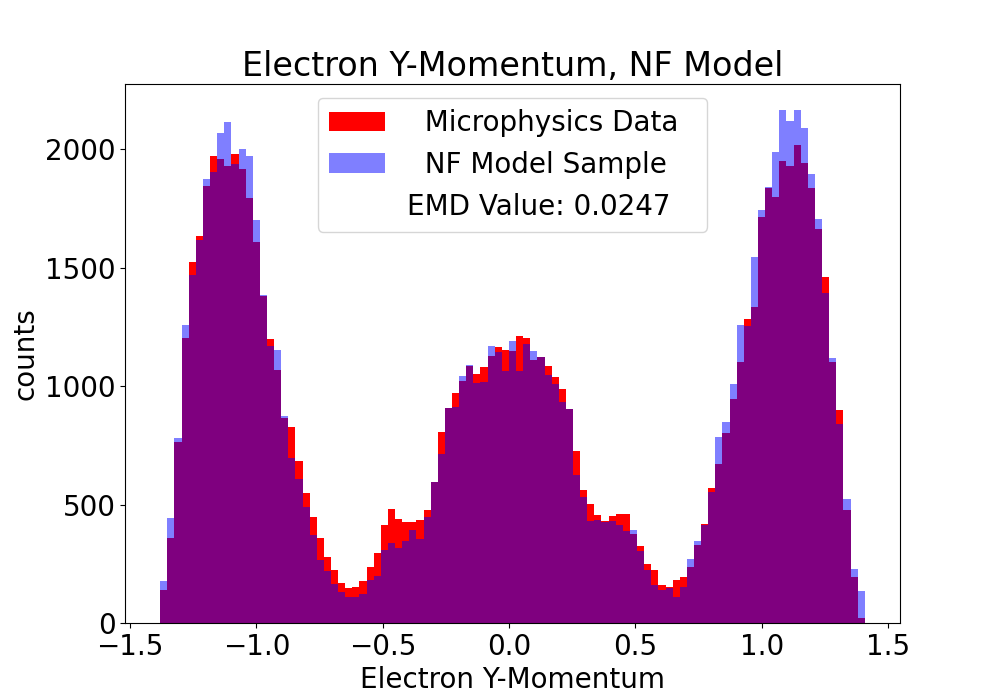
\includegraphics[width=.97\textwidth]{images/Features16/Electron_Y-Momentum,_NF_Model.png}
            \end{figure}
    \end{columns}
\end{frame}


\begin{frame}{Results: Comparing Generated and Test Distributions}
   \begin{columns}
            \column{0.3\textwidth}
            Proton Features
            \begin{itemize}
                    \setlength\itemsep{0.3em}
                    \item Energy tails are difficult to match exactly
                    \item Momenta mostly well reproduced
            \end{itemize}
   
            \column{0.3\textwidth}
            \begin{figure}[H]
            \centering
            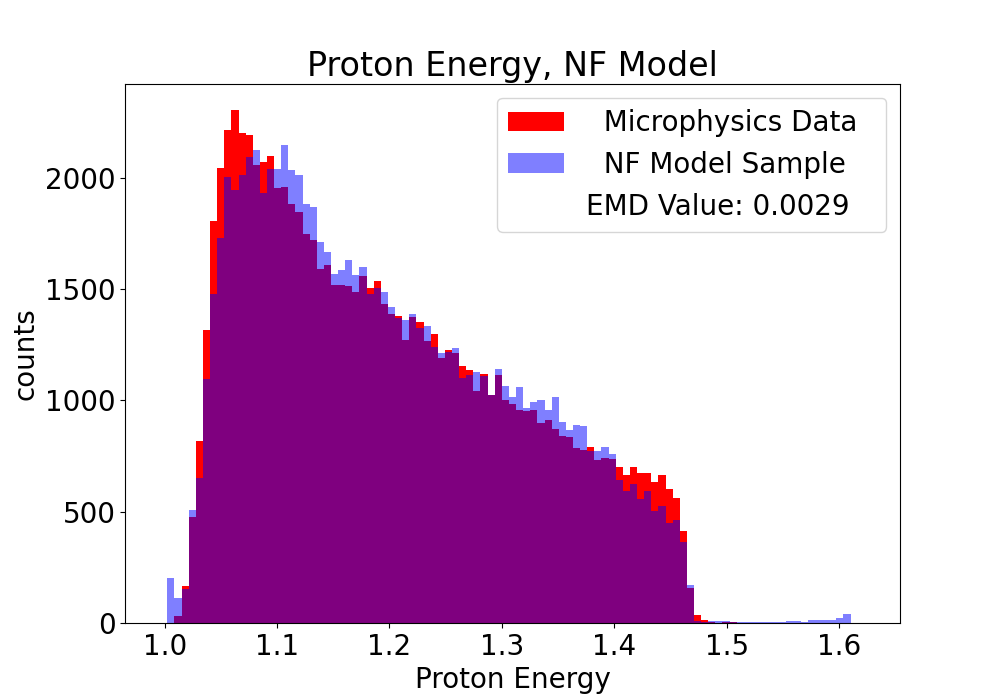
\includegraphics[width=.97\textwidth]{images/Features16/Proton_Energy,_NF_Model.png}
            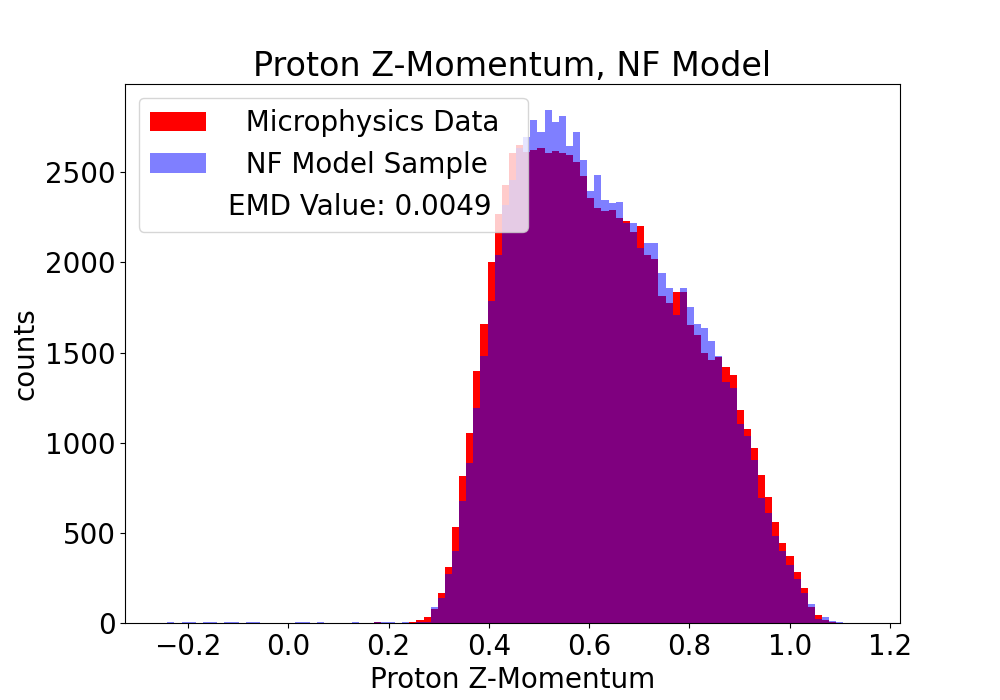
\includegraphics[width=.97\textwidth]{images/Features16/Proton_Z-Momentum,_NF_Model.png}
            \label{fig:clas6}
            \end{figure}
            
             \column{0.3\textwidth}
             \begin{figure}[H]
            \centering
            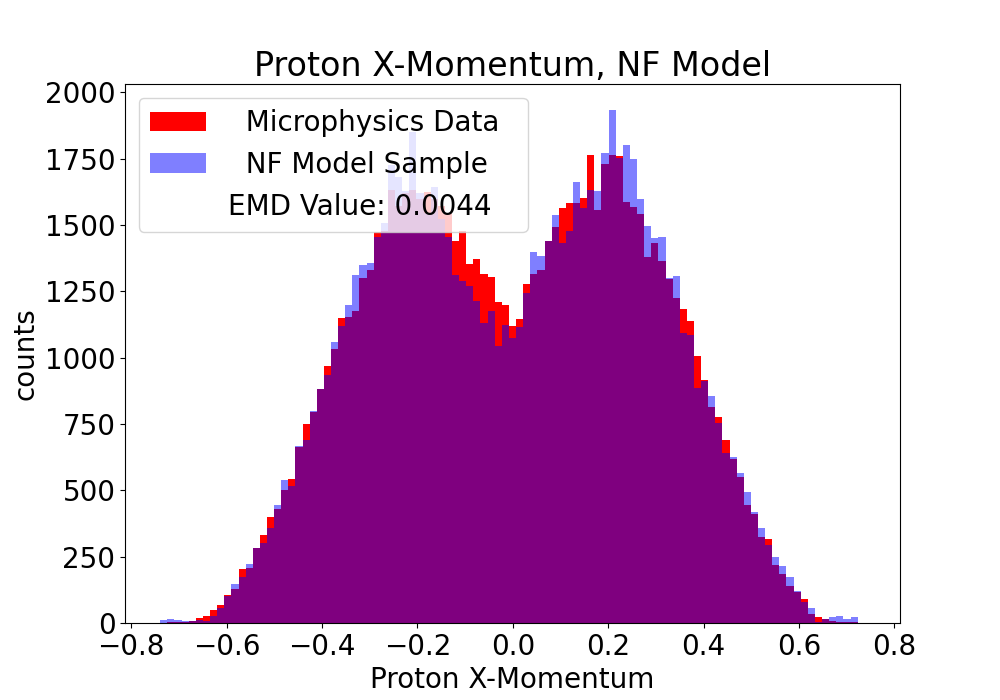
\includegraphics[width=.97\textwidth]{images/Features16/Proton_X-Momentum,_NF_Model.png}
            \includegraphics[width=.97\textwidth]{images/Features16/Proton_Y-Momentum,_NF_Model.png}
            \end{figure}
    \end{columns}
\end{frame}


\begin{frame}{Results: Comparing Generated and Test Distributions}
   \begin{columns}
            \column{0.3\textwidth}
            Photon 1 Features
            \begin{itemize}
                    \setlength\itemsep{0.3em}
                    \item NF mostly reproduced the distributions well
                    \item Small discrepancies on transverse momenta peaks
            \end{itemize}
   
            \column{0.3\textwidth}
            \begin{figure}[H]
            \centering
            \includegraphics[width=.97\textwidth]{images/Features16/Photon_1_Energy,_NF_Model.png}
            \includegraphics[width=.97\textwidth]{images/Features16/Photon_1_Z-Momentum,_NF_Model.png}
            \label{fig:clas6}
            \end{figure}
            
             \column{0.3\textwidth}
             \begin{figure}[H]
            \centering
            \includegraphics[width=.97\textwidth]{images/Features16/Photon_1_X-Momentum,_NF_Model.png}
            \includegraphics[width=.97\textwidth]{images/Features16/Photon_1_Y-Momentum,_NF_Model.png}
            \end{figure}
    \end{columns}
\end{frame}


\begin{frame}{Results: Comparing Generated and Test Distributions}
   \begin{columns}
            \column{0.3\textwidth}
            Photon 2 Features
            \begin{itemize}
                    \setlength\itemsep{0.3em}
                    \item Lower energy than photon 1
                    \item NF oversamples low energy/momenta
            \end{itemize}
   
            \column{0.3\textwidth}
            \begin{figure}[H]
            \centering
            \includegraphics[width=.97\textwidth]{images/Features16/Photon_2_Energy,_NF_Model.png}
            \includegraphics[width=.97\textwidth]{images/Features16/Photon_2_Z-Momentum,_NF_Model.png}
            \label{fig:clas6}
            \end{figure}
            
             \column{0.3\textwidth}
             \begin{figure}[H]
            \centering
            \includegraphics[width=.97\textwidth]{images/Features16/Photon_2_X-Momentum,_NF_Model.png}
            \includegraphics[width=.97\textwidth]{images/Features16/Photon_2_Y-Momentum,_NF_Model.png}
            \end{figure}
    \end{columns}
\end{frame}


\begin{frame}{Use Earth Mover's Distance to Evaluate Distribution Similarity}
    \begin{columns}
    \column{0.7\textwidth}
Informally, interpret two distribution samples as two different ways of piling up the same amount of dirt over a region, then the EMD is the minimum cost of turning one pile into the other; where the cost is assumed to be amount of dirt moved times the distance by which it is moved.

Computationally complex, for simple 1D distributions can be calculated by the Wasserstein-1 metric.


 
 %https://stats.stackexchange.com/questions/295617/what-is-the-advantages-of-wasserstein-metric-compared-to-kullback-leibler-diverg
 
 
 \column{0.3\textwidth}
 
 \begin{figure}[!h]
    \centering
    %\includegraphics[scale=0.3]{FinalPictures/EMD/EmdRatio.png}
    \includegraphics[width=.99\textwidth,trim={2.5cm 1.75cm 2cm 2.1cm},clip]{images/EMDSample.png}
    \label{fig:EMD}
\end{figure}
Identical distributions have EMD=0, 2 finite samples drawn from the same distribution have small nonzero EMD.

    \end{columns}
\small
%\vspace{1cm}
wikipedia.org/wiki/Earth\_mover\%27s\_distance

\end{frame}


\begin{frame}{NF Model EMD $\sim$ 5x Worse than Ideal Case}
Red reference line is EMD value between 2 samples from physics test dataset; blue points are EMD values for each feature
\begin{figure}[!h]
    \centering
    %\includegraphics[scale=0.3]{FinalPictures/EMD/EmdRatio.png}
    \includegraphics[width=.6\textwidth,trim={2.5cm 1.75cm 2cm 2.1cm},clip]{images/EMD/nflow_emd_with_text.png}
    \label{fig:EMD}
\end{figure}
\end{frame}

\begin{frame}{Comparison of 2D Feature Distributions Shows Discrepancies}
NF Models are having a difficult time learning the sharp feature cutoffs caused by conservation laws and physics detector layout
\begin{figure}[!ht]
  
    \begin{minipage}{.2\textwidth}
        
        Physics Data\\
        
        \vspace{1cm}
        
  
        NF Model\\
    \end{minipage}%
    \begin{minipage}{.2573\textwidth}
    
        \centering
       % Electron
        \includegraphics[width=0.95\textwidth,trim={0 0 0 0},clip]{images/Hists2D/Proton_P_X_vs_Photon_1_P_Z,_Physics_Data.png}
        \includegraphics[width=0.95\textwidth,trim={0 0 0 0},clip]{images/Hists2D/Proton_P_X_vs_Photon_1_P_Z,_NF_Model.png}

        %\caption{(c)}
    \end{minipage}%
    \begin{minipage}{0.2573\textwidth}
        \centering
       %Feature Distributions from Traditional Microphysics Simulations
        \includegraphics[width=0.95\textwidth,trim={0 0 0 0},clip]{images/Hists2D/Electon_P_X_vs_Proton_P_X,_Physics_Data.png}
        %Feature Distributions from NF Model Samples
        \includegraphics[width=0.95\textwidth,trim={0 0 0 0},clip]{images/Hists2D/Electon_P_X_vs_Proton_P_X,_NF_Model.png}
        %\caption{(a)}
        

    \end{minipage}
     \begin{minipage}{0.2573\textwidth}
            \centering
           % Photon 1
            \includegraphics[width=0.95\textwidth,trim={0 0 0 0},clip]{images/Hists2D/Electon_P_X_vs_Electron_P_Y,_Physics_Data.png}
            \includegraphics[width=0.95\textwidth,trim={0 0 0 0},clip]{images/Hists2D/Electon_P_X_vs_Electron_P_Y,_NF_Model.png}

    \end{minipage}
    \label{fig:2D}
\end{figure}
\end{frame}

\begin{frame}{4-Feature NF Model Produces Better Results}
   \begin{columns}
            \column{0.3\textwidth}
           Trained Model with only 4 Features
            \begin{itemize}
                    \setlength\itemsep{0.3em}
                    \item Observe better reproduction of fine detail
                    \item Still not extremely high fidelity
                    \item Model now much more limited in scope
            \end{itemize}
   
            \column{0.3\textwidth}
            \begin{figure}[H]
            \centering
            \includegraphics[width=.97\textwidth]{images/2D_Hists_4F/Electon_P_X_vs_Electron_P_Y,_Physics_Data.png}
            \includegraphics[width=0.97\textwidth,trim={0 0 0 0},clip]{images/Hists2D/Electon_P_X_vs_Electron_P_Y,_NF_Model.png}
            
            
            \label{fig:clas6}
            \end{figure}
            
             \column{0.3\textwidth}
             \begin{figure}[H]
            \centering
            \includegraphics[width=.97\textwidth]{images/2D_Hists_4F/Electon_P_X_vs_Electron_P_Y,_NF_4-Feature_Model.png}
            \includegraphics[width=.97\textwidth]{images/2D_Hists_4F/Electron_P_X_vs_P_Y,_NF_4-Feat_Model,_M_e2_Cut.png}
            
            \end{figure}
    \end{columns}
\end{frame}

\begin{frame}{4-Feature NF Model EMD Values Also Better}
EMD values for 4-feature model are considerably lower than those measured in the 16-feature model
\begin{figure}[!h]
    \centering
    %\includegraphics[scale=0.3]{FinalPictures/EMD/EmdRatio.png}
    \includegraphics[scale=0.35]{images/EMD/emdratio416.png}
    \label{fig:EMD}
\end{figure}
\end{frame}

\begin{frame}{16-Feature Model Yields Meaningful Physics Quantities}
The 16-feature model performs well enough to be able to observe various particle masses embedded in the physics process; this information is not accessible in a 4-feature model
   \begin{columns}

            \column{0.45\textwidth}
            \begin{figure}[H]
            \centering
            \includegraphics[width=.87\textwidth]{images/RecoMass/protons}
            \label{fig:clas6}
            \end{figure}
            
             \column{0.45\textwidth}
             \begin{figure}[H]
            \centering
            \includegraphics[width=.87\textwidth]{images/RecoMass/pions}
            \end{figure}
    \end{columns}

\end{frame}

\begin{frame}{Conclusions and Path Forward}
    \begin{itemize}
        \item Used UMNN-MAF architecture to train NF model to produce physics event distributions
        \item Can sample from the trained NF $\sim$ 10-100 times faster than current simulation methods
        \item 16-Feature model works well enough to reproduce physics quantities of interest, but important discrepancies still remain
        \item Work is ongoing to incorporate physics and physical symmetries and constraints to improve training
    \end{itemize}
\end{frame}



\iffalse

\begin{frame}{Conclusions and Path Forward}
    \begin{itemize}
        
    
    
    
    
        \item Used normalizing flows to obtain reasonable physics distributions far faster than traditional physics simulations
        \item 4-feature model provides much greater resolution and speed-up compared with 16-feature case, single particle modelling can still be useful for study of background processes at CLAS12
        \item Implementing conservation laws into training to improve model resolution
        \item Optimizing model to generate sample faster
    \end{itemize}
\end{frame}

\fi

\end{document}
